\chapter{La glucosa de la sangre y la diabetes}\label{ch:g12:glucose-and-diabetes}

Cinco litros de sangre, un gramo de glucosa en cada uno: cinco gramos
en total, más o menos un terrón de azúcar. Solo el cerebro quema esa
cantidad cada hora, de día y de noche, y no puede usar ninguna otra
cosa. Y sin embargo, una persona que no come nada en todo un día, o que
se come una tarta entera de una vez, mantiene la concentración a unas
pocas décimas de gramo por litro del mismo valor --- y una persona a la
que le ha fallado el páncreas no lo consigue, con consecuencias que van
de la sed al coma. Este capítulo trata del número más vigilado del
organismo, de los órganos que lo mantienen estable y de lo que pasa, en
las dos formas de la \omterm{def:g12:glucose-and-diabetes:diabetes}{diabetes}, cuando no pueden.

\section{Una constante regulada}

\begin{definition}[Glucemia]\label{def:g12:glucose-and-diabetes:glycaemia}
La \emph{glucemia}\index{glucemia} es la concentración de glucosa en el
plasma sanguíneo: alrededor de \qty{1}{g/L} (\qty{5.5}{mmol/L}) antes
de una comida en una persona sana, con una subida a \qty{1.4}{g/L} en
la hora siguiente a comer y una vuelta al valor de partida en dos, y
una bajada a \qty{0.7}{g/L} tras un día de ayuno. Por debajo de
\qty{0.5}{g/L} el cerebro falla (confusión y después coma); por encima
de \qty{1.8}{g/L} la glucosa se derrama a la orina, y años por encima
de \qty{1.3}{g/L} dañan los vasos y los nervios. La glucemia es una
magnitud \emph{regulada}: un valor mantenido cerca de una consigna por
un sistema que lo mide y lo corrige.
\end{definition}

\begin{proposition}[La reserva de glucosa y sus flujos]\label{prop:g12:glucose-and-diabetes:pool}
Los \qty{5}{g} de glucosa de la sangre son una reserva por la que pasan
flujos grandes. \emph{Entradas}: el intestino después de una comida
(hasta \qty{100}{g} en una hora) y, entre comidas, el \emph{hígado},
que suelta glucosa de su \emph{\omterm{def:g10:exercise-and-energy:glycogen}{glucógeno}} almacenado (\qty{100}{g},
medio día de suministro) y fabrica glucosa nueva a partir de
\omterm{def:g10:chemistry-of-life:families}{aminoácidos} y de lactato. \emph{Salidas}: el cerebro (\qty{5}{g/h},
constante), los músculos (de unos pocos gramos a \qty{100}{g/h} en
trabajo), otros tejidos, y el almacenamiento como \omterm{def:g10:exercise-and-energy:glycogen}{glucógeno} en el
hígado y los músculos o como grasa. Una reserva de \qty{5}{g}
alimentada y vaciada a decenas de gramos por hora solo es estable
porque los flujos se ajustan minuto a minuto.
\end{proposition}
\admitted

\begin{omfigure}
\begin{tikzpicture}[font=\small, >=Stealth,
  b/.style={draw, rounded corners, align=center, minimum height=1.0cm}]
  \node[b, fill=omThm!15, text width=3.0cm, minimum height=1.6cm] (blood) at (0,0) {glucosa de la sangre\\ \qty{5}{g}, unos \qty{1}{g/L}};
  \node[b, fill=omDef!12, text width=2.6cm] (gut) at (-4.5,1.6) {intestino\\ (tras las comidas)};
  \node[b, fill=omDef!12, text width=2.6cm] (liver) at (-4.5,-1.6) {hígado: reserva de\\ glucógeno, glucosa nueva};
  \node[b, fill=omMeth!15, text width=2.6cm] (brain) at (4.5,1.6) {cerebro: \qty{5}{g/h},\\ solo glucosa};
  \node[b, fill=omMeth!15, text width=2.6cm] (muscle) at (4.5,0) {músculos: la usan y la\\ guardan como glucógeno};
  \node[b, fill=omMeth!15, text width=2.6cm] (fat) at (4.5,-1.6) {tejido adiposo:\\ la guarda como grasa};
  \draw[->, thick] (gut) -- (blood.west |- 0,0.5);
  \draw[<->, thick] (liver) -- node[below=1pt, font=\scriptsize, sloped] {en los dos sentidos} (blood.west |- 0,-0.5);
  \draw[->, thick] (blood.east |- 0,0.5) -- (brain);
  \draw[->, thick] (blood.east) -- (muscle);
  \draw[->, thick] (blood.east |- 0,-0.5) -- (fat);
\end{tikzpicture}

{\small La reserva de glucosa. Las comidas y el hígado la alimentan; el
cerebro, los músculos y el tejido adiposo la vacían; solo el hígado
puede trabajar en los dos sentidos, almacenando después de una comida y
soltando entre comidas.}
\end{omfigure}

\begin{example}[Un día de glucemia]\label{ex:g12:glucose-and-diabetes:day}
Desayuno a las 8: la \omterm{def:g12:glucose-and-diabetes:glycaemia}{glucemia} sube de \num{0.9} a \qty{1.3}{g/L} a las
9 y vuelve a \num{1.0} a las 10, con el exceso ido al \omterm{def:g10:exercise-and-energy:glycogen}{glucógeno} del
hígado y de los músculos. De 10 a 13, el hígado suelta \omterm{def:g10:exercise-and-energy:glycogen}{glucógeno} y el
nivel se mantiene cerca de \num{0.9}. Una carrera a las 17 lleva
\qty{60}{g} a los músculos en una hora; el hígado vacía la mitad de su
reserva para seguirle el ritmo, y el nivel baja a \num{0.8}. Por la
noche, el hígado fabrica glucosa nueva a partir de \omterm{def:g10:chemistry-of-life:families}{aminoácidos}, y a las
7 el nivel es de \qty{0.9}{g/L}. Trescientos gramos han pasado por una
reserva de cinco.
\end{example}

\section{El páncreas mantiene el equilibrio}

\begin{proposition}[Dos hormonas de los islotes]\label{prop:g12:glucose-and-diabetes:hormones}
Repartidos por el páncreas, entre las \omterm{def:g10:cells-common-unit:cell}{células} que fabrican \omterm{def:g11:enzymes-and-phenotype:enzyme}{enzimas}
digestivas, hay un millón de agrupaciones pequeñas de \omterm{def:g10:cells-common-unit:cell}{células}, los
\emph{islotes}\index{islotes del páncreas}. Sus \omterm{def:g10:cells-common-unit:cell}{células} miden la
\omterm{def:g12:glucose-and-diabetes:glycaemia}{glucemia} de la sangre que pasa y secretan en ella dos \omterm{def:g11:hormones-and-reproduction:hormone}{hormonas}:
\begin{itemize}
  \item la \emph{insulina}\index{insulina}, de las \omterm{def:g10:cells-common-unit:cell}{células} $\beta$,
        cuando la \omterm{def:g12:glucose-and-diabetes:glycaemia}{glucemia} sube: hace que las \omterm{def:g10:cells-common-unit:cell}{células} musculares y
        adiposas capten glucosa, y que el hígado y los músculos la
        almacenen como \omterm{def:g10:exercise-and-energy:glycogen}{glucógeno}; la \omterm{def:g12:glucose-and-diabetes:glycaemia}{glucemia} baja;
  \item el \emph{glucagón}\index{glucagón}, de las \omterm{def:g10:cells-common-unit:cell}{células} $\alpha$,
        cuando baja: hace que el hígado degrade el \omterm{def:g10:exercise-and-energy:glycogen}{glucógeno} y suelte
        glucosa; la \omterm{def:g12:glucose-and-diabetes:glycaemia}{glucemia} sube.
\end{itemize}
Las dos actúan sobre los mismos órganos en sentidos contrarios; su
equilibrio, reajustado cada pocos minutos por la \omterm{def:g12:glucose-and-diabetes:glycaemia}{glucemia} medida, es la
regulación. La \omterm{prop:g12:glucose-and-diabetes:hormones}{insulina} es la única \omterm{def:g11:hormones-and-reproduction:hormone}{hormona} que baja la \omterm{def:g12:glucose-and-diabetes:glycaemia}{glucemia};
varias la suben.
\end{proposition}
\begin{proof}[Pruebas experimentales]
Quitarle el páncreas a un perro (1889) lo vuelve diabético en un día:
su \omterm{def:g12:glucose-and-diabetes:glycaemia}{glucemia} se triplica y aparece glucosa en su orina; ligar el
conducto que lleva las \omterm{def:g11:enzymes-and-phenotype:enzyme}{enzimas} digestivas no lo hace, así que el efecto
no es digestivo. Inyectar un extracto de los \omterm{prop:g12:glucose-and-diabetes:hormones}{islotes} (1921) baja la
\omterm{def:g12:glucose-and-diabetes:glycaemia}{glucemia} de un perro diabético, y la de un niño diabético, en unas
horas; la sustancia activa, la \omterm{prop:g12:glucose-and-diabetes:hormones}{insulina}, se purificó ese mismo año.
Unos \omterm{prop:g12:glucose-and-diabetes:hormones}{islotes} aislados en una placa secretan \omterm{prop:g12:glucose-and-diabetes:hormones}{insulina} cuando se sube la
glucosa del medio y \omterm{prop:g12:glucose-and-diabetes:hormones}{glucagón} cuando se baja. El \omterm{prop:g12:glucose-and-diabetes:hormones}{glucagón} inyectado sube
la \omterm{def:g12:glucose-and-diabetes:glycaemia}{glucemia} de una persona en ayunas en unos minutos, y solo si el
hígado tiene \omterm{def:g10:exercise-and-energy:glycogen}{glucógeno}.
\end{proof}

\begin{omfigure}
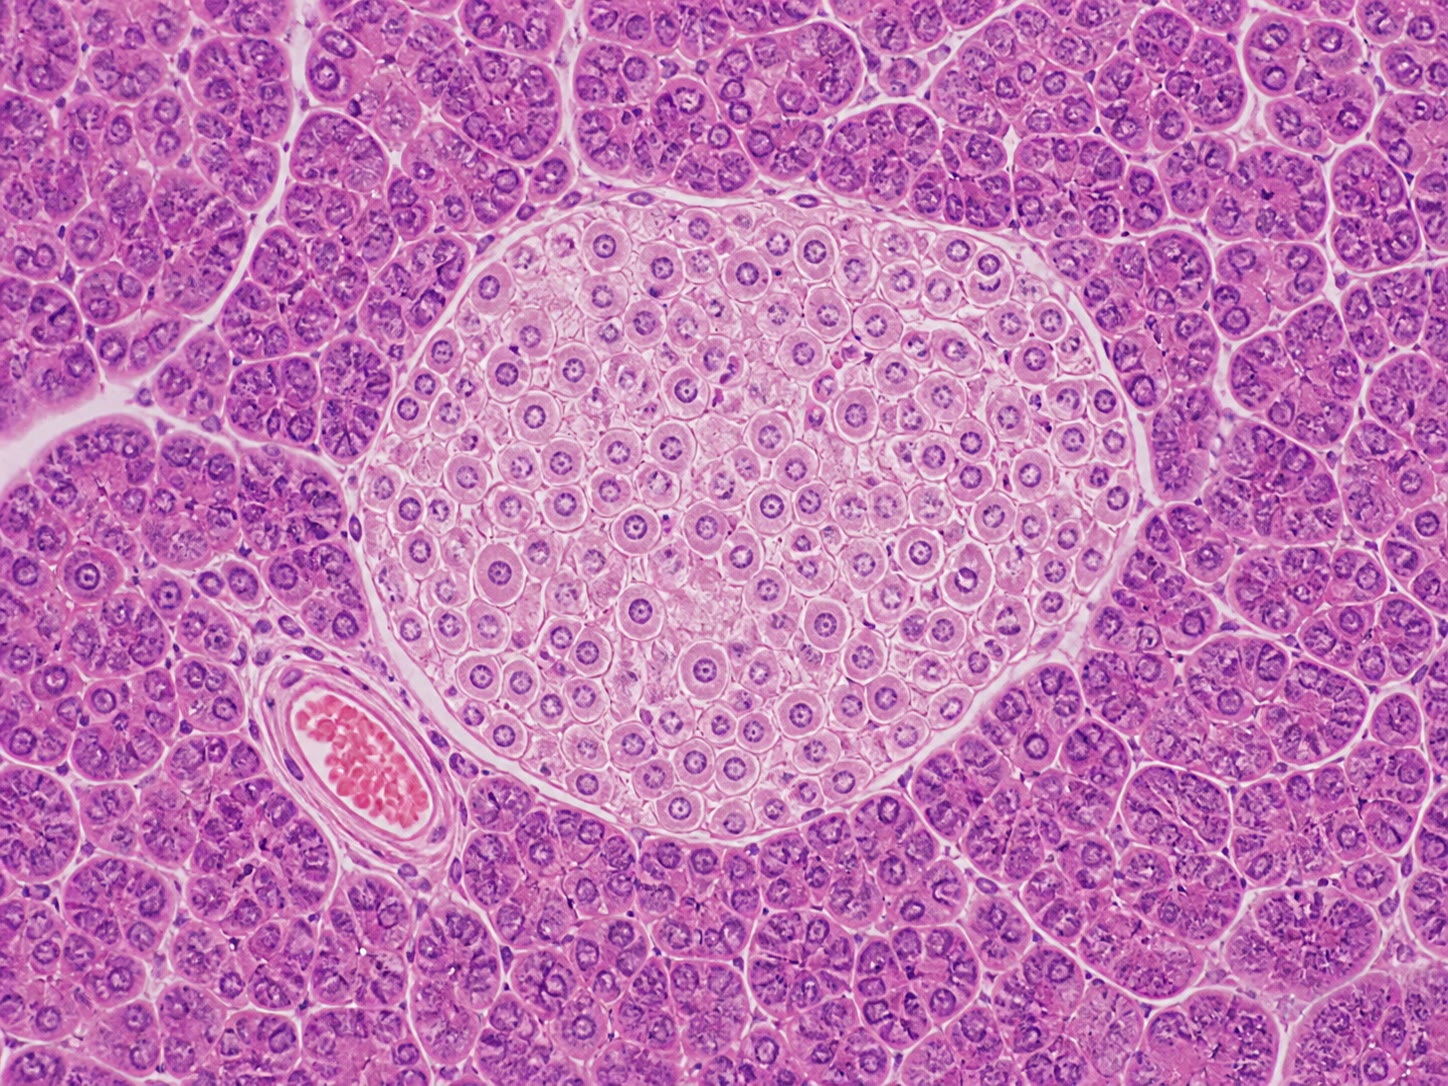
\includegraphics[width=0.56\linewidth]{images/book2/ai/g12-glucose-pancreas-islet.jpg}

{\small Un corte de páncreas: un islote, más pálido, entre las
agrupaciones más oscuras de las \omterm{def:g10:cells-common-unit:cell}{células} que secretan \omterm{def:g11:enzymes-and-phenotype:enzyme}{enzimas}. Las
\omterm{def:g10:cells-common-unit:cell}{células} del islote leen la glucosa de la sangre y responden con
\omterm{prop:g12:glucose-and-diabetes:hormones}{insulina} o con \omterm{prop:g12:glucose-and-diabetes:hormones}{glucagón}; el resto del órgano fabrica jugo digestivo.}
\end{omfigure}

\begin{omfigure}
\begin{tikzpicture}[font=\small, >=Stealth,
  b/.style={draw, rounded corners, align=center, minimum height=1.0cm}]
  \node[b, fill=omThm!15, text width=3.2cm, minimum height=1.4cm] (gly) at (0,0) {glucemia\\ (consigna \qty{1}{g/L})};
  \node[b, fill=omProp!15, text width=2.8cm] (beta) at (-4.6,2.0) {células $\beta$: insulina};
  \node[b, fill=omProp!15, text width=2.8cm] (alpha) at (-4.6,-2.0) {células $\alpha$: glucagón};
  \node[b, fill=omMeth!15, text width=3.4cm] (store) at (5.6,2.2) {hígado, músculo, grasa:\\ captan y almacenan glucosa};
  \node[b, fill=omMeth!15, text width=3.4cm] (rel) at (5.6,-2.2) {hígado: degrada el\\ glucógeno, suelta glucosa};
  \draw[->, thick] (gly.west |- 0,0.4) -- node[above, sloped, font=\scriptsize] {subida detectada} (beta.east);
  \draw[->, thick] (gly.west |- 0,-0.4) -- node[below, sloped, font=\scriptsize] {bajada detectada} (alpha.east);
  \draw[->, thick, omProp] (beta.north) -- ++(0,0.6) -| (store.north);
  \draw[->, thick, omProp] (alpha.south) -- ++(0,-0.6) -| (rel.south);
  \draw[->, thick, omThm] (store.west) -- node[above, sloped, font=\scriptsize, align=center] {la glucemia\\ baja $(-)$} (gly.east |- 0,0.4);
  \draw[->, thick, omThm] (rel.west) -- node[below, sloped, font=\scriptsize, align=center] {la glucemia\\ sube $(+)$} (gly.east |- 0,-0.4);
  \node[font=\scriptsize, anchor=south] at (0,3.3) {insulina};
  \node[font=\scriptsize, anchor=north] at (0,-3.3) {glucagón};
\end{tikzpicture}

{\small La regulación de la \omterm{def:g12:glucose-and-diabetes:glycaemia}{glucemia}. Una subida dispara la \omterm{prop:g12:glucose-and-diabetes:hormones}{insulina},
que hace que los tejidos almacenen glucosa y baja el nivel; una bajada
dispara el \omterm{prop:g12:glucose-and-diabetes:hormones}{glucagón}, que hace que el hígado suelte glucosa y lo sube.
El efecto de cada \omterm{def:g11:hormones-and-reproduction:hormone}{hormona} suprime la señal que la llamó: dos bucles de
\omterm{def:g11:hormones-and-reproduction:hormone}{retroalimentación} negativa alrededor de una sola consigna.}
\end{omfigure}

\begin{example}[El bucle en acción]\label{ex:g12:glucose-and-diabetes:loop}
Después de una comida, la \omterm{def:g12:glucose-and-diabetes:glycaemia}{glucemia} trepa; en unos minutos, las \omterm{def:g10:cells-common-unit:cell}{células}
$\beta$ sueltan \omterm{prop:g12:glucose-and-diabetes:hormones}{insulina}, las \omterm{def:g10:cells-common-unit:cell}{células} musculares y adiposas abren sus
transportadores de glucosa, el hígado se pone a fabricar \omterm{def:g10:exercise-and-energy:glycogen}{glucógeno} y el
nivel vuelve a bajar --- momento en el que la secreción de \omterm{prop:g12:glucose-and-diabetes:hormones}{insulina}
baja también. Entre comidas, la deriva hacia abajo la contrarresta el
\omterm{prop:g12:glucose-and-diabetes:hormones}{glucagón}, el \omterm{def:g10:exercise-and-energy:glycogen}{glucógeno} se degrada y el nivel se mantiene. Ninguna de
las dos \omterm{def:g11:hormones-and-reproduction:hormone}{hormonas} falta nunca; lo que se mueve es su proporción, y la
\omterm{def:g12:glucose-and-diabetes:glycaemia}{glucemia} la sigue dentro de una banda estrecha.
\end{example}

\section{Cuando el bucle falla: la diabetes}

\begin{definition}[Diabetes]\label{def:g12:glucose-and-diabetes:diabetes}
La \emph{diabetes}\index{diabetes} es un exceso crónico de \omterm{def:g12:glucose-and-diabetes:glycaemia}{glucemia}:
por encima de \qty{1.26}{g/L} en ayunas, o por encima de \qty{2}{g/L}
dos horas después de una carga estándar de glucosa. Sus primeros signos
se siguen del exceso: glucosa en la orina, que arrastra agua consigo
(orina abundante, sed), y pérdida de peso cuando las \omterm{def:g10:cells-common-unit:cell}{células} no pueden
usar la glucosa que las rodea. Sus daños tardíos --- a los vasos
pequeños del \omterm{def:g11:the-eye:parts}{ojo} y del riñón, a los nervios, a las arterias --- vienen
de años de glucosa reaccionando con las \omterm{def:g10:chemistry-of-life:families}{proteínas}. Dos enfermedades
comparten el nombre.
\end{definition}

\begin{proposition}[Tipo 1 y tipo 2]\label{prop:g12:glucose-and-diabetes:types}
\begin{itemize}
  \item La \emph{\omterm{def:g12:glucose-and-diabetes:diabetes}{diabetes} de tipo 1} (alrededor del 10\% de los casos)
        es la destrucción de las \omterm{def:g10:cells-common-unit:cell}{células} $\beta$ por el propio sistema
        inmunitario del paciente, casi siempre en la infancia o en la
        juventud: la \omterm{prop:g12:glucose-and-diabetes:hormones}{insulina} falta. La \omterm{def:g12:glucose-and-diabetes:glycaemia}{glucemia} sube sin freno, se
        quema grasa a falta de glucosa utilizable y sus productos
        ácidos se acumulan; sin \omterm{prop:g12:glucose-and-diabetes:hormones}{insulina} inyectada, la enfermedad es
        mortal en unos meses. El tratamiento es \omterm{prop:g12:glucose-and-diabetes:hormones}{insulina}, varias veces
        al día, dosificada según las comidas y la \omterm{def:g12:glucose-and-diabetes:glycaemia}{glucemia} medida, de
        por vida.
  \item La \emph{\omterm{def:g12:glucose-and-diabetes:diabetes}{diabetes} de tipo 2} (alrededor del 90\%) aparece en
        adultos, casi siempre con sobrepeso y sedentarios: los tejidos
        responden cada vez menos a la \omterm{prop:g12:glucose-and-diabetes:hormones}{insulina} (\emph{resistencia a la
        \omterm{prop:g12:glucose-and-diabetes:hormones}{insulina}}), las \omterm{def:g10:cells-common-unit:cell}{células} $\beta$ lo compensan secretando más y,
        al cabo de unos años, se agotan. La \omterm{prop:g12:glucose-and-diabetes:hormones}{insulina} está presente,
        pero es insuficiente. La predisposición es en parte genética
        (\cref{ch:g11:genes-and-disease}); el desencadenante es el modo
        de vida, y el primer tratamiento es cambiarlo --- perder peso y
        hacer ejercicio --- antes que los medicamentos y, tarde, la
        \omterm{prop:g12:glucose-and-diabetes:hormones}{insulina}.
\end{itemize}
\end{proposition}
\begin{proof}[Pruebas experimentales]
Los pacientes de tipo 1 tienen anticuerpos contra sus propias \omterm{def:g10:cells-common-unit:cell}{células}
de los \omterm{prop:g12:glucose-and-diabetes:hormones}{islotes} años antes de los síntomas y, en el momento del
diagnóstico, sus \omterm{prop:g12:glucose-and-diabetes:hormones}{islotes} están casi vacíos de \omterm{def:g10:cells-common-unit:cell}{células} $\beta$ e
infiltrados de glóbulos blancos; su \omterm{prop:g12:glucose-and-diabetes:hormones}{insulina} en sangre es indetectable
y responden a la \omterm{prop:g12:glucose-and-diabetes:hormones}{insulina} inyectada de inmediato. Los pacientes de tipo
2 tienen una \omterm{prop:g12:glucose-and-diabetes:hormones}{insulina} normal o alta en el momento del diagnóstico; sus
\omterm{def:g10:cells-common-unit:cell}{células} musculares y adiposas captan menos glucosa para una misma dosis
de \omterm{prop:g12:glucose-and-diabetes:hormones}{insulina} que las de una persona sana; los gemelos idénticos
comparten la enfermedad en el 70\% de los casos, y perder peso o
seguir un programa de caminatas restablece por sí solo una \omterm{def:g12:glucose-and-diabetes:glycaemia}{glucemia}
normal en muchos casos precoces.
\end{proof}

\begin{omfigure}
\begin{tikzpicture}
\begin{axis}[
  width=0.88\linewidth, height=5.8cm,
  axis x line=bottom, axis y line=left,
  xmin=0, xmax=180, ymin=0, ymax=3,
  xlabel={minutos tras beber \qty{75}{g} de glucosa}, ylabel={glucemia (g/L)},
  xlabel style={font=\small, at={(axis description cs:0.5,-0.12)}, anchor=north},
  ylabel style={font=\small},
  tick label style={font=\small}, xtick={0,30,60,90,120,150,180}, ytick={0,1,2,3},
  legend style={at={(0.5,-0.3)}, anchor=north, legend columns=3, font=\small, draw=none},
  clip=false,
]
\addplot[thick, omMeth, smooth] coordinates {(0,0.9) (30,1.4) (60,1.3) (90,1.1) (120,0.95) (150,0.9) (180,0.9)};
\addplot[thick, omProp, smooth] coordinates {(0,1.1) (30,1.7) (60,1.9) (90,1.85) (120,1.7) (150,1.5) (180,1.35)};
\addplot[thick, omThm, smooth] coordinates {(0,1.6) (30,2.3) (60,2.7) (90,2.8) (120,2.7) (150,2.6) (180,2.5)};
\draw[dashed, gray] (axis cs:0,2) -- (axis cs:180,2);
\node[font=\scriptsize, gray, anchor=south east] at (axis cs:180,2.02) {umbral a los 120 min};
\legend{sana, tolerancia alterada, diabetes de tipo 2}
\end{axis}
\end{tikzpicture}

{\small La prueba de tolerancia a la glucosa: la \omterm{def:g12:glucose-and-diabetes:glycaemia}{glucemia} tras una
bebida estándar de \qty{75}{g} de glucosa. Una persona sana vuelve
cerca de \qty{1}{g/L} en dos horas; una diabética empieza alta, trepa
por encima de \qty{2}{g/L} y se queda ahí. La curva intermedia es la
fase de aviso, casi siempre reversible.}
\end{omfigure}

\begin{example}[Sacar adelante un día con tipo 1]\label{ex:g12:glucose-and-diabetes:type1}
Una adolescente con tipo 1 se mide la \omterm{def:g12:glucose-and-diabetes:glycaemia}{glucemia} antes de cada comida con
una gota de sangre, cuenta los hidratos de carbono de su plato y se
inyecta una dosis de \omterm{prop:g12:glucose-and-diabetes:hormones}{insulina} rápida proporcional a ellos --- una
unidad por cada \qty{10}{g}, más o menos ---, además de una \omterm{prop:g12:glucose-and-diabetes:hormones}{insulina}
lenta una vez al día para el fondo. Con demasiada \omterm{prop:g12:glucose-and-diabetes:hormones}{insulina}, o si se
salta una comida, el nivel baja de \qty{0.6}{g/L}: sudores, temblores,
confusión, que se corrigen con azúcar en unos minutos. Con demasiado
poca, el nivel se queda por encima de \qty{2}{g/L}, con sed y fatiga, y
los vasos van encajando el daño en silencio. Ella hace, a mano, lo que
sus \omterm{def:g10:cells-common-unit:cell}{células} $\beta$ hacían por \omterm{def:g11:hormones-and-reproduction:hormone}{retroalimentación}.
\end{example}

\begin{omfigure}
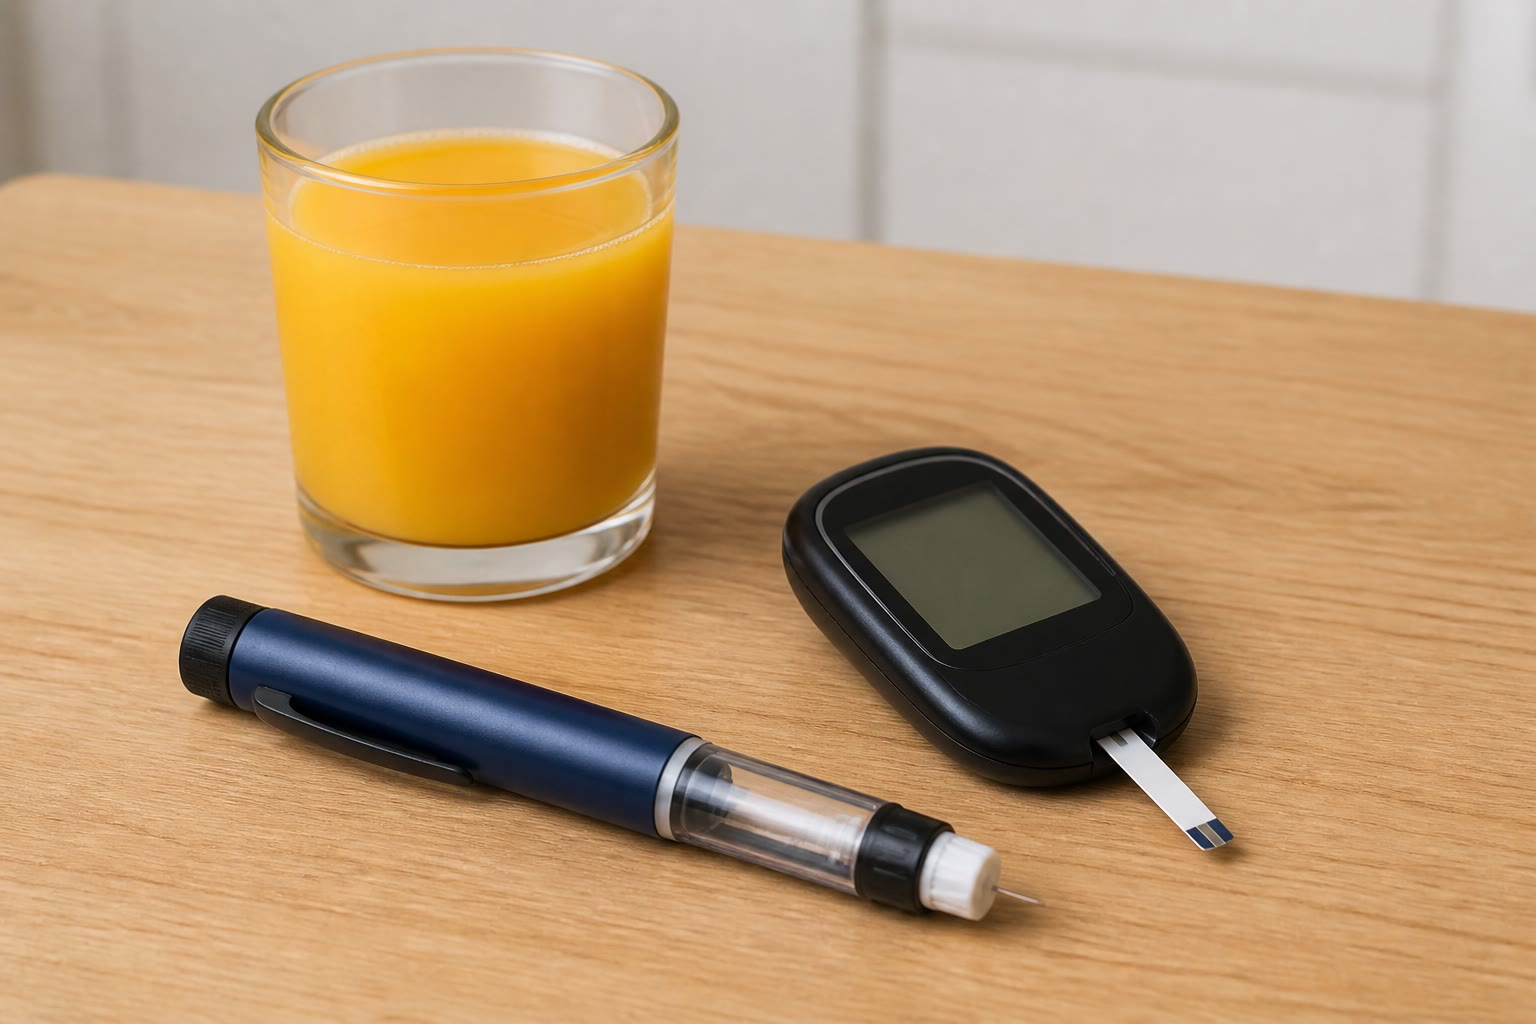
\includegraphics[width=0.56\linewidth]{images/book2/ai/g12-glucose-meter-pen.jpg}

{\small Los útiles de una diabética de tipo 1: un medidor que lee la
\omterm{def:g12:glucose-and-diabetes:glycaemia}{glucemia} de una gota de sangre y una pluma que inyecta una dosis medida
de \omterm{prop:g12:glucose-and-diabetes:hormones}{insulina}. El bucle de los \omterm{prop:g12:glucose-and-diabetes:hormones}{islotes}, ejecutado a mano varias veces al
día.}
\end{omfigure}

\begin{method}[Leer un registro de glucemia]\label{met:g12:glucose-and-diabetes:read}
\begin{enumerate}
  \item Localiza la consigna y la banda: en ayunas
        \qtyrange{0.7}{1.1}{g/L}, tras las comidas por debajo de
        \num{1.4}; dos horas después de una carga de glucosa, por
        debajo de \num{1.4} (sana), \qtyrange{1.4}{2}{} (alterada),
        por encima de \qty{2}{g/L} (\omterm{def:g12:glucose-and-diabetes:diabetes}{diabetes}).
  \item Para cada subida, pregúntate qué metió glucosa (una comida, el
        hígado) y qué debería sacarla (las dianas de la \omterm{prop:g12:glucose-and-diabetes:hormones}{insulina}); para
        cada bajada, qué la sacó (el cerebro, el músculo) y qué debería
        reponerla (el \omterm{prop:g12:glucose-and-diabetes:hormones}{glucagón}, el hígado).
  \item Lee las \omterm{def:g11:hormones-and-reproduction:hormone}{hormonas} junto con la glucosa: la \omterm{prop:g12:glucose-and-diabetes:hormones}{insulina} debería
        subir con la \omterm{def:g12:glucose-and-diabetes:glycaemia}{glucemia} y el \omterm{prop:g12:glucose-and-diabetes:hormones}{glucagón} bajar; una \omterm{prop:g12:glucose-and-diabetes:hormones}{insulina} ausente
        significa tipo 1, y una \omterm{prop:g12:glucose-and-diabetes:hormones}{insulina} alta con una \omterm{def:g12:glucose-and-diabetes:glycaemia}{glucemia} alta
        significa resistencia.
  \item Convierte las unidades cuando haga falta: \qty{1}{g/L} de
        glucosa son \qty{5.55}{mmol/L}.
\end{enumerate}
\end{method}

\begin{remark}[Un modelo de regulación]\label{rem:g12:glucose-and-diabetes:model}
Sensor, consigna, dos efectores opuestos, \omterm{def:g11:hormones-and-reproduction:hormone}{retroalimentación} negativa:
el control de la \omterm{def:g12:glucose-and-diabetes:glycaemia}{glucemia} tiene el mismo diseño que el control de la
\omterm{prop:g11:becoming-male-female:hormones}{testosterona} del \cref{ch:g11:hormones-and-reproduction}, y que el
diseño de casi todas las constantes del organismo --- la temperatura,
el agua, la presión arterial, la acidez. La \omterm{def:g12:glucose-and-diabetes:diabetes}{diabetes} es el aspecto que
tiene una constante regulada cuando su bucle está roto: el valor sigue
respondiendo a las entradas, pero nada lo devuelve a su sitio. Leer las
curvas de este capítulo es entrenarse para leer cualquiera de ellas.
\end{remark}

\section{Ejercicios}

\begin{exercise}[$\star$]\label{exo:g12:glucose-and-diabetes:1}
Da la \omterm{def:g12:glucose-and-diabetes:glycaemia}{glucemia} normal en ayunas en \unit{g/L} y en \unit{mmol/L}, y los
dos umbrales de peligro.
\end{exercise}

\begin{exercise}[$\star$]\label{exo:g12:glucose-and-diabetes:2}
Nombra las dos \omterm{def:g11:hormones-and-reproduction:hormone}{hormonas} de los \omterm{prop:g12:glucose-and-diabetes:hormones}{islotes}, las \omterm{def:g10:cells-common-unit:cell}{células} que las fabrican y
el efecto de cada una sobre la \omterm{def:g12:glucose-and-diabetes:glycaemia}{glucemia}.
\end{exercise}

\begin{exercise}[$\star$]\label{exo:g12:glucose-and-diabetes:3}
¿Qué órgano puede almacenar y soltar glucosa? ¿En qué forma la
almacena?
\end{exercise}

\begin{exercise}[$\star$]\label{exo:g12:glucose-and-diabetes:4}
Enuncia en una frase cada una la diferencia esencial entre la \omterm{def:g12:glucose-and-diabetes:diabetes}{diabetes}
de tipo 1 y la de tipo 2.
\end{exercise}

\begin{exercise}[$\star$]\label{exo:g12:glucose-and-diabetes:5}
En la figura de la prueba de tolerancia, lee las tres curvas a los 120
minutos y clasifica cada una.
\end{exercise}

\begin{exercise}[$\star\star$]\label{exo:g12:glucose-and-diabetes:6}
El cerebro usa \qty{5}{g} de glucosa por hora y la sangre contiene
\qty{5}{g}. Explica por qué una persona no pierde el conocimiento una
hora después de una comida, y nombra el órgano y la \omterm{def:g11:hormones-and-reproduction:hormone}{hormona}
responsables.
\end{exercise}

\begin{exercise}[$\star\star$]\label{exo:g12:glucose-and-diabetes:7}
Explica por qué quitar el páncreas provoca \omterm{def:g12:glucose-and-diabetes:diabetes}{diabetes} pero ligar su
conducto no, y qué muestra esto sobre dónde se fabrica la \omterm{prop:g12:glucose-and-diabetes:hormones}{insulina} y
cómo viaja.
\end{exercise}

\begin{exercise}[$\star\star$]\label{exo:g12:glucose-and-diabetes:8}
Una persona en ayunas recibe una inyección de \omterm{prop:g12:glucose-and-diabetes:hormones}{glucagón}: la \omterm{def:g12:glucose-and-diabetes:glycaemia}{glucemia}
sube \qty{0.4}{g/L} en 20 minutos. La misma inyección tras tres días de
ayuno no hace nada. Explícalo.
\end{exercise}

\begin{exercise}[$\star\star$]\label{exo:g12:glucose-and-diabetes:9}
¿Por qué una persona diabética orina en abundancia y tiene sed?
\end{exercise}

\begin{exercise}[$\star\star$]\label{exo:g12:glucose-and-diabetes:10}
Una paciente de tipo 1 se inyecta su dosis habitual de \omterm{prop:g12:glucose-and-diabetes:hormones}{insulina} y luego
se salta la comida. Predice qué pasa en las dos horas siguientes y por
qué.
\end{exercise}

\begin{exercise}[$\star\star$]\label{exo:g12:glucose-and-diabetes:11}
Explica por qué el ejercicio baja la \omterm{def:g12:glucose-and-diabetes:glycaemia}{glucemia} de una persona con
\omterm{def:g12:glucose-and-diabetes:diabetes}{diabetes} de tipo 2 incluso sin ningún cambio de \omterm{prop:g12:glucose-and-diabetes:hormones}{insulina}, con ayuda del
\cref{ch:g10:sport-and-health}.
\end{exercise}

\begin{exercise}[$\star\star\star$]\label{exo:g12:glucose-and-diabetes:12}
Dos pacientes tienen una \omterm{def:g12:glucose-and-diabetes:glycaemia}{glucemia} en ayunas de \qty{2}{g/L}. Uno no
tiene \omterm{prop:g12:glucose-and-diabetes:hormones}{insulina} detectable; el otro tiene tres veces la \omterm{prop:g12:glucose-and-diabetes:hormones}{insulina} normal.
Diagnostica a cada uno, y di qué están haciendo los \omterm{prop:g12:glucose-and-diabetes:hormones}{islotes} de cada
paciente.
\end{exercise}

\begin{exercise}[$\star\star\star$]\label{exo:g12:glucose-and-diabetes:13}
Dibuja, o describe, las curvas de la \omterm{def:g12:glucose-and-diabetes:glycaemia}{glucemia} y de la \omterm{prop:g12:glucose-and-diabetes:hormones}{insulina} en las
tres horas siguientes a una comida en una persona sana, en un paciente
de tipo 1 sin tratamiento y en un paciente de tipo 2. Explica cada
diferencia.
\end{exercise}

\begin{exercise}[$\star\star\star$]\label{exo:g12:glucose-and-diabetes:14}
Una comida contiene \qty{80}{g} de hidratos de carbono. Si todos
entraran de golpe en la sangre, ¿en cuánto se quedaría la \omterm{def:g12:glucose-and-diabetes:glycaemia}{glucemia}?
Explica por qué eso no pasa nunca, y enumera los destinos de la glucosa
en las dos primeras horas.
\end{exercise}

\begin{exercise}[$\star\star\star$]\label{exo:g12:glucose-and-diabetes:15}
Compara la regulación de la \omterm{def:g12:glucose-and-diabetes:glycaemia}{glucemia} con la de la \omterm{prop:g11:becoming-male-female:hormones}{testosterona} del
\cref{ch:g11:hormones-and-reproduction}: sensor, consigna, efectores,
signo de la \omterm{def:g11:hormones-and-reproduction:hormone}{retroalimentación}. ¿Qué tiene de especial disponer de dos
\omterm{def:g11:hormones-and-reproduction:hormone}{hormonas} opuestas?
\end{exercise}

\section{Problema: Cinco gramos de azúcar}

\begin{problem}[{Problema de fin de semana --- la glucosa de la sangre
contabilizada a lo largo de un día: la reserva y sus flujos, una prueba
de tolerancia leída, una dosis de insulina calculada y un bucle que hay
que sustituir a mano}]
\label{pb:g12:glucose-and-diabetes:1}
Toma un volumen de sangre de \qty{5}{L}, un consumo cerebral de
\qty{5}{g/h} de glucosa, una reserva de \omterm{def:g10:exercise-and-energy:glycogen}{glucógeno} hepático de
\qty{100}{g} y un \omterm{def:g10:exercise-and-energy:glycogen}{glucógeno} muscular de \qty{400}{g}. Una unidad de
\omterm{prop:g12:glucose-and-diabetes:hormones}{insulina} rápida se ocupa de unos \qty{10}{g} de hidratos de carbono.

\medskip
\noindent\textbf{Parte I --- La reserva.}
\begin{enumerate}
  \item Calcula la masa de glucosa de la sangre a \qty{1}{g/L}, y esa
        misma concentración en \unit{mmol/L} (glucosa
        \qty{180}{g/mol}).
  \item ¿Cuánto le duraría al cerebro solo la glucosa de la sangre, si
        nada la repusiera?
  \item Entre comidas, el hígado la repone. ¿Cuánto le dura al cerebro
        el \omterm{def:g10:exercise-and-energy:glycogen}{glucógeno} del hígado? ¿Qué pasa después?
  \item El \omterm{def:g10:exercise-and-energy:glycogen}{glucógeno} muscular es cuatro veces el del hígado, pero los
        músculos no pueden soltar glucosa a la sangre. Explica por qué
        el \omterm{def:g10:exercise-and-energy:glycogen}{glucógeno} muscular no ayuda al cerebro, y para qué sirve.
  \item Una comida entrega \qty{60}{g} de glucosa a lo largo de una
        hora. Si no se retirara nada, ¿a cuánto llegaría la \omterm{def:g12:glucose-and-diabetes:glycaemia}{glucemia}?
        ¿Qué la retira en realidad, y adónde va?
\end{enumerate}

\medskip
\noindent\textbf{Parte II --- La prueba.}
Un paciente bebe \qty{75}{g} de glucosa. \omterm{def:g12:glucose-and-diabetes:glycaemia}{Glucemia} e \omterm{prop:g12:glucose-and-diabetes:hormones}{insulina} medidas:

\begin{center}
\begin{tabular}{lcccccc}
minutos & 0 & 30 & 60 & 90 & 120 & 180 \\ \hline
\omterm{def:g12:glucose-and-diabetes:glycaemia}{glucemia} (g/L) & 1.15 & 1.8 & 2.05 & 2.0 & 1.85 & 1.6 \\
\omterm{prop:g12:glucose-and-diabetes:hormones}{insulina} (\% de un máximo sano) & 90 & 140 & 180 & 200 & 190 & 160 \\
\end{tabular}
\end{center}
\begin{enumerate}[resume]
  \item Clasifica al paciente con los umbrales del
        \cref{met:g12:glucose-and-diabetes:read}.
  \item ¿Falta \omterm{prop:g12:glucose-and-diabetes:hormones}{insulina}? ¿Qué es entonces lo que falla?
  \item Nombra la enfermedad, y da dos rasgos que esperarías de la
        historia del paciente.
  \item ¿Qué aspecto tendría esa misma tabla en un paciente de tipo 1
        sin tratamiento?
  \item ¿Cuál es el primer tratamiento que se prescribe, y por qué
        mecanismo actúa?
\end{enumerate}

\medskip
\noindent\textbf{Parte III --- Ejecutar el bucle a mano.}
La \omterm{def:g12:glucose-and-diabetes:glycaemia}{glucemia} de una paciente de tipo 1 es de \qty{1.0}{g/L} antes de
cenar; la comida contiene \qty{90}{g} de hidratos de carbono.
\begin{enumerate}[resume]
  \item Calcula la dosis de \omterm{prop:g12:glucose-and-diabetes:hormones}{insulina} rápida para la comida.
  \item Se la inyecta pero solo se come la mitad de la cena. Estima
        cuánto puede bajar la \omterm{def:g12:glucose-and-diabetes:glycaemia}{glucemia}, y nombra los síntomas y el
        remedio.
  \item No se inyecta nada y se come la cena entera. Estima la \omterm{def:g12:glucose-and-diabetes:glycaemia}{glucemia}
        si los \qty{90}{g} entraran todos en una reserva de \qty{5}{L},
        y di qué hacen los riñones por encima de \qty{1.8}{g/L}.
  \item ¿Por qué tiene que inyectarse además una \omterm{prop:g12:glucose-and-diabetes:hormones}{insulina} lenta por la
        noche, cuando no come nada?
  \item Explica en qué sentido el medidor y la pluma sustituyen a la
        \omterm{def:g10:cells-common-unit:cell}{célula} $\beta$, y qué no pueden sustituir.
\end{enumerate}

\medskip
\noindent\textbf{Parte IV --- El bucle, razonado.}
\begin{enumerate}[resume]
  \item Un medicamento estimula a las \omterm{def:g10:cells-common-unit:cell}{células} $\beta$ para que secreten
        más \omterm{prop:g12:glucose-and-diabetes:hormones}{insulina}. ¿En qué tipo de \omterm{def:g12:glucose-and-diabetes:diabetes}{diabetes} puede funcionar, y por
        qué no en el otro?
  \item Una persona con tipo 2 pierde \qty{10}{kg} y camina una hora al
        día; seis meses después, la prueba de tolerancia es normal.
        Explica qué parte del bucle se ha reparado.
  \item Explica por qué en una persona sana la \omterm{prop:g12:glucose-and-diabetes:hormones}{insulina} y el \omterm{prop:g12:glucose-and-diabetes:hormones}{glucagón}
        nunca están los dos altos, y qué hace un islote en una placa
        cuando la glucosa del medio se fija en \qty{1}{g/L}.
  \item El \omterm{prop:g12:glucose-and-diabetes:hormones}{glucagón}, la \omterm{prop:g10:heart-lungs-effort:control}{adrenalina}, el cortisol y la \omterm{def:g11:hormones-and-reproduction:hormone}{hormona} del
        crecimiento suben todos la \omterm{def:g12:glucose-and-diabetes:glycaemia}{glucemia}; solo la \omterm{prop:g12:glucose-and-diabetes:hormones}{insulina} la baja.
        Propón por qué el organismo tiene varias salvaguardas contra
        una \omterm{def:g12:glucose-and-diabetes:glycaemia}{glucemia} baja y una sola contra una alta.
  \item Enuncia el resultado: la glucosa de la sangre, las horas que
        puede cubrir el hígado, el diagnóstico de la parte II y la
        dosis de la parte III.
\end{enumerate}
\end{problem}
